\chapter{設計}\label{chap:design}

本章では、本研究で提案するプログラミング環境の設計について述べる。

\section{設計指針}\label{ux8a2dux8a08ux6307ux91dd}

第\ref{chap:background}章では、プログラムの処理領域と処理実行対象について述べ、新しいプログラミング環境の必要性について述べた。
現状の仕組みでは、既存のプログラミング言語上で具体的な人物を対象とした、
人間と計算機の融合型のプログラムを記述・実行することはできない。
そこで、本章ではこのようなプログラムを記述・実行できる環境の設計と検討を行う。

特定の人物を計算機と同じようにプログラムから利用出来るようにするためには以下の要素が必要である。

\begin{itemize}
\itemsep1pt\parskip0pt\parsep0pt
\item
  プログラム上での対象人物の指定
\item
  プログラムから人への処理内容の伝達
\item
  人からプログラムへの処理結果の伝達
\end{itemize}

加えて、必要に応じて人間と計算機を切り替えて利用できるよう、可能な限り類似の記法にて実現する必要がある。
また、人間とプログラムのインタフェースとして機能するソフトウェアが必要となる。
様々なデバイスや既存ソフトウェア上で、インタフェースとなるソフトウェアを動作させることが出来れば有用である。
この際、デバイスごとに仕様が異なる可能性や、
既存ソフトウェア上で動かす場合は、そのソフトウェアの仕様に沿った実装をしなくてはいけないという点を考慮する必要がある。
インタフェースとなるソフトウェアを実装しやすくするために、外部の仕様に左右されやすい部分を
換装が容易に可能なモジュールとして設計する。
これらの点について、以下の節にて詳しく設計を述べる。

\section{プログラムと人間のインタラクション設計}\label{sec:program-human-interaction-design}

\subsection{プログラムと人間のメッセージ交換モデル}\label{ux30d7ux30edux30b0ux30e9ux30e0ux3068ux4ebaux9593ux306eux30e1ux30c3ux30bbux30fcux30b8ux4ea4ux63dbux30e2ux30c7ux30eb}

プログラムと人間のインタラクションを実現するためには、
プログラムと人間がメッセージを交換できるようなモデルの構築が必要となる。
このモデルを構築するため、従来のプログラムとコンピュータの関係を応用する。

従来のプログラムでは、書かれている処理を実行する対象はコンピュータであり、
コンピュータはプログラムに書かれている内容に忠実に従い、処理を行う。
これは、プログラムからの処理命令をコンピュータがメッセージとして受け取り、そのメッセージの通りに処理を
実行したその結果をプログラムに送るという、プログラムとコンピュータのメッセージ交換であると言える。

このモデルをそのまま人間にも適応する。
つまり、プログラムからの処理命令を人間がメッセージとして受け取り、人間はそのメッセージ通りに処理を行う。
そして、実行した結果をプログラムに送る。
このメッセージ交換モデルを構築することが出来れば、プログラムと人間のインタラクションが実現すると言える。

しかし、現状では、プログラムから人間に直接メッセージを送る仕組みは存在しない。
その逆も同じで、人間からプログラムへと直接メッセージを送ることも出来ない。
そこで、本研究においては、
インターネット接続していてメッセージを受信可能なデバイスを仲介することによって、
デバイス経由で人間にメッセージを送る。
つまり、デバイスを経由して指示内容を伝え、デバイスを経由して処理結果を入力させるという、
デバイス仲介型のプログラムと人間のメッセージ交換モデルを採用する。

このようなプログラムと人間のインタラクションを実現することによって、
プログラムから人間にアクセスできるようにし、計算資源として扱えるようにする。

\subsection{具体的な人間の指定}\label{ux5177ux4f53ux7684ux306aux4ebaux9593ux306eux6307ux5b9a}

既存の仕組みでは、具体的な人物を指定し、プログラム上で計算資源として活用することはできない。
これは、主に人間の演算能力に注目しその能力を活かすことが既存の仕組みの目的であったからだ。
そのため、クラウドソーシングのプラットフォームの利用が前提となっており、具体的な人間を指定することができなかった。
しかし、本研究では人間の実世界のタスクの処理能力にも注目しているため、具体的な人物の指定が必須となる。
例えば、自分の家におけるタスクを処理するためには、自分や家族を指定することが望まれる。

\begin{figure}[htbp]
  \begin{center}
  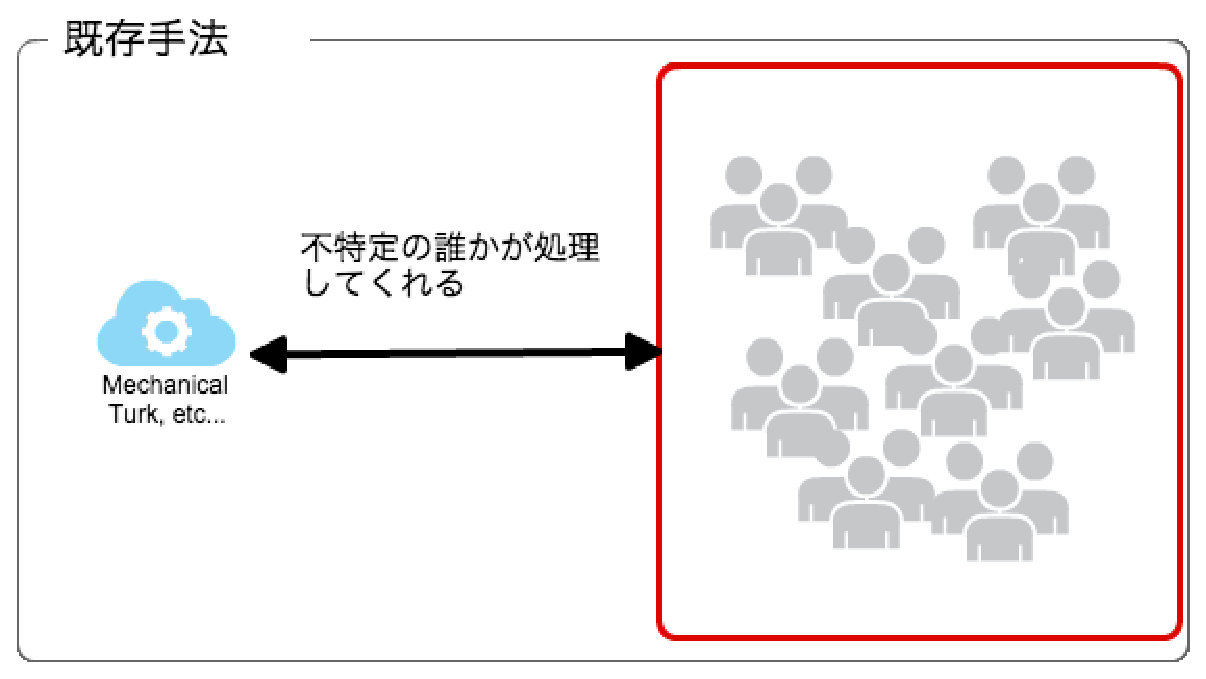
\includegraphics[width=.5\linewidth]{images/crowdsourcing_model.eps}
  \end{center}
  \caption{クラウドソーシングのモデル}
  \label{fig:crowdsourcing_model}
\end{figure}

そこで、プログラム上に人間をオブジェクトとして扱えるようにし、そのオブジェクトの宣言時にidを指定することで、
そのidを持った人間に指示を送るような仕組みを採用することで、具体的に人物を指定した指示を実現する。
また、このオブジェクトへのメッセージングは人間へのメッセージングとして解釈する。
このような仕組みを実装することによって、具体的な人間を指定したプログラムと人間のインタラクションの実現させる。

\begin{figure}[htbp]
  \begin{center}
  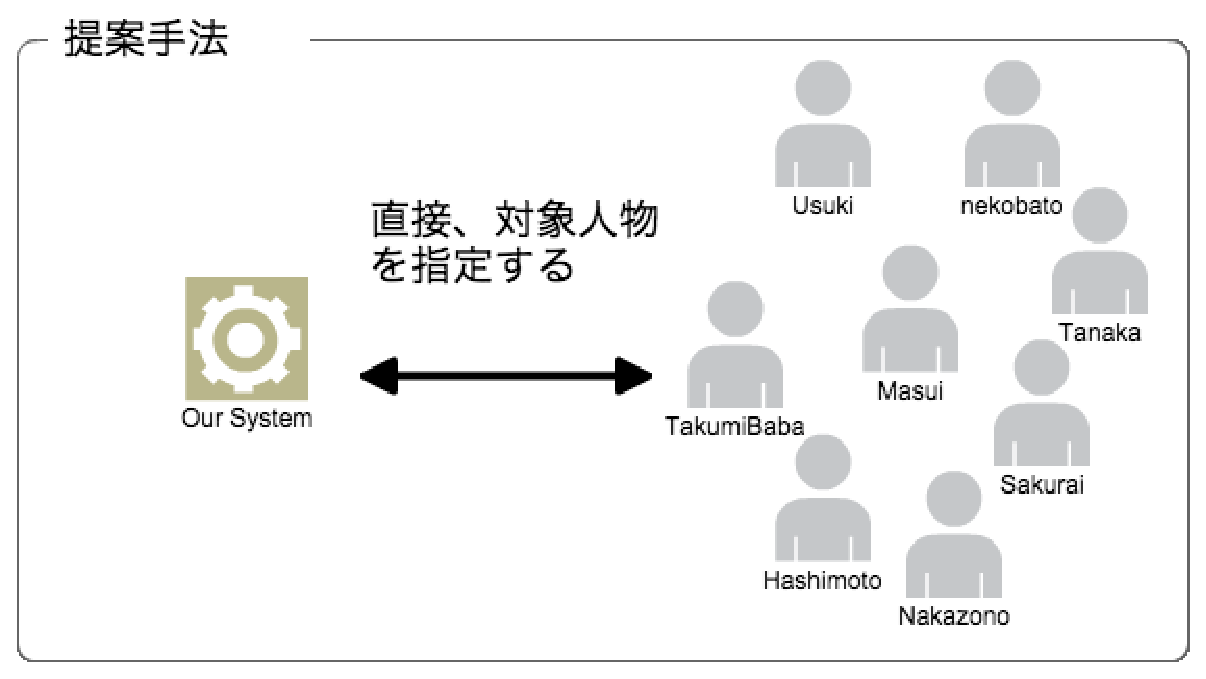
\includegraphics[width=.5\linewidth]{images/unique_id_model.eps}
  \end{center}
  \caption{提案手法のモデル}
  \label{fig:unique_id_model}
\end{figure}

\subsection{統一的な記法}\label{ux7d71ux4e00ux7684ux306aux8a18ux6cd5}

人間への指示を既存のプログラムと同じような記法で実現させる。
同等の記述によって人間への指示を実現させることによって、人間と計算機を使った処理の切り替えを容易に記述できるようにする。
本研究では、ある処理を実現する上で、計算機でも出来ることならば計算機に、人間がやったほうが良い場合や、人間にしかできないようなことは
人間に実行させるのが望ましいという考えを前提としている。
そのため、状況に応じて両者への指示を切り替えられるようなプログラムが記述できるようにする必要がある。
例えば、ロボットでも出来そうな処理ならばロボットに実行させ、人間は感性を必要とする判断等、人間にしか出来ないことに
専念すべきであるが、もしロボットがなければ人間に実行させるといったことが実現可能であるべきだ。

上記のようなことの実現は現在の仕組みでは難しい。
例えば、データベースに問い合わせ、保存されているデータを取得するプログラムでの記述と同じような記法で
人間に問い合わせ、データを取得するようなプログラムが記述できるべきである。
データベースに情報があるならば、データベースに問い合わせる処理を実行すれば良いし、
ないならば、人間に問い合わせれば良い(ソースコード:\ref{code:design-integrated-program-style})。

\begin{lstlisting}[caption=人間への指示を計算機への指示と類似させる, label=code:design-integrated-program-style]
// データベース問い合わせの擬似コード
new db('tasks').find({id: 1}, function(err, doc){

});
// 人間への問い合わせの擬似コード
new Human('takumibaba').find({message: ''}, function(err, result){

});
\end{lstlisting}

同様に、センサーを利用して部屋の温度を取得するプログラムの記述と同じような記法で
人間を利用して、部屋のセンシングに利用するようなプログラムが記述できるべきだ。
センサーが部屋にないならば、人間に問い合わせれば良い。
これらの処理の切り替えを容易に記述できるようにするためには、可能な限り類似の記法を踏襲する必要がある。

\subsection{人間とプログラムのインタフェース}\label{ux4ebaux9593ux3068ux30d7ux30edux30b0ux30e9ux30e0ux306eux30a4ux30f3ux30bfux30d5ux30a7ux30fcux30b9}

前節までの設計に関する考察のように、人間とプログラムのメッセージングによって
両者のインタラクションを実現するためには、人間とプログラムのインタフェースとして機能するソフトウェアの実装が必要である。
プログラムからの指示をユーザに提示し、処理を促し、何かしらの結果を入力するまでの一連の流れを担うものであり、
一種のソフトウェアエージェントとして動作する。

必要な実装要件としては、以下の通りである。

\begin{itemize}
\itemsep1pt\parskip0pt\parsep0pt
\item
  指示内容の提示
\item
  実行結果の入力フォームの提示
\end{itemize}

上記内容、特に実行結果の入力フォームの提示における工夫をすることで、人間への負担を減らすように設計する必要がある。
まず、入力する情報の限定などが考えられる。
例えば、プログラム側で求めている結果が、Boolean型であるならばtrueかfalseを返すようなインタフェースのみを提示すべきである。
また、指示内容に従えない場合や現実との乖離から実行出来ない場合などに放置するということがないよう、
エラーを返すことのできるような仕組みを取り入れる必要がある。

このような、人間とプログラムの間を仲介するソフトウェアエージェントの実装をすることは、人間とプログラムのインタラクションの
実現に不可欠である。

\section{プラガブルなモジュール構成}\label{sec:plaggable-module-design}

前述の通り、様々なデバイスやメディア上でプログラムと人間のインタフェースとなるソフトウェアを実装・運用可能にする必要がある。
だが、近年ではデバイスは多様化しており、その仕様も大きくことなる。
例えば、パソコンやスマートフォンではユーザに提示すべきインタフェースの設計が異なる。
画面の大きさの違いはそのままインタフェースの設計に影響を与える。
また、通信手法も異なることが多い。
パソコンであれば、基本的に常時コネクションを張り続けるといったことが可能であるが、スマートフォンの場合は
コネクションを切られてしまうこともある。

こういった状況を考慮して、デバイス依存しやすい部分については、交換が容易に可能なモジュールとして設計する必要がある。
交換可能なモジュールとして設計することで、デバイスごとに依存部分のプログラムを書くだけで、
共通部分の再実装をする必要がなくなる。
また、応用アプリケーション等の実装も容易となる、

本研究では、デバイス依存が強いと考えている以下の2点に関して、特別なモジュールとして扱う。

\begin{itemize}
\itemsep1pt\parskip0pt\parsep0pt
\item
  通信手法
\item
  ユーザインタフェース
\end{itemize}

通信手法は各デバイスごとに異なるため、選択可能であることが望ましい。
可能ならば、プログラムとデバイスが常にコネクションを貼り続け、いつでもリアルタイムに通信が出来る状態にしておくことが良いが、
リアルタイム通信が実現出来ない状況も存在する。
例えばスマートフォンの場合はOSによっては、一定時間の経過もしくはアプリケーションがバックグラウンド処理に回された際に
リアルタイム通信を切断をすることがある。
移動中等、通信状況が安定しない場合も考えられ、一つの通信手法に縛られず、様々な手法を利用できることが望ましい。

提示すべきユーザインタフェースも交換可能にしておくべきである。
スクリーンサイズの問題や、何かしらの既存ソフトウェア上に実装する場合には
ユーザインタフェースはその仕様に合うように提示すべきである。

また、上記の2点以外の部分に関しても、プラグインという形で拡張が可能になるような実装を行う。

\section{新しいプログラミング環境の要件のまとめ}\label{ux65b0ux3057ux3044ux30d7ux30edux30b0ux30e9ux30dfux30f3ux30b0ux74b0ux5883ux306eux8981ux4ef6ux306eux307eux3068ux3081}

前節までの設計検討から、人間と計算機への指示を融合させた新しいプログラミング環境の要件についてまとめる。
まず、\ref{sec:program-human-interaction-design}節から、
プログラム上で人間とのインタラクションを可能にするプログラムモジュールと、
プログラムと人間の仲介となるソフトウェアエージェントが必要となる。
前者のプログラムモジュールは、具体的な人間を指定可能で、既存のプログラミングスタイルを踏襲して
人間への指示を送り、その実行結果を得ることが出来る。
後者のソフトウェアエージェントでは、指示に対して人間が値を返しやすいようなユーザインタフェースを提供し、
プログラムと人間の間の情報のやりとりをサポートする。

次に、\ref{sec:plaggable-module-design}節から、主にソフトウェアエージェントを運用するデバイスや
既存アプリケーションごとに異なる可能性の高い仕様の部分に関しては、容易に実装が可能で、交換できる
モジュールになるよう設計し、実装する。
拡張性を可能な限り高め、関連するプログラムの実装を容易にすることが目的である。

これらをまとめて、人間と計算への指示を融合させたプログラミング環境として提案する。
次章では、このプログラミング環境の各要素について詳しく述べる。
